\chapter{Data Exploration}
\label{chapter:data}
\section{EU-Forest Labels}

\begin{figure}[!thb]
    \centering
    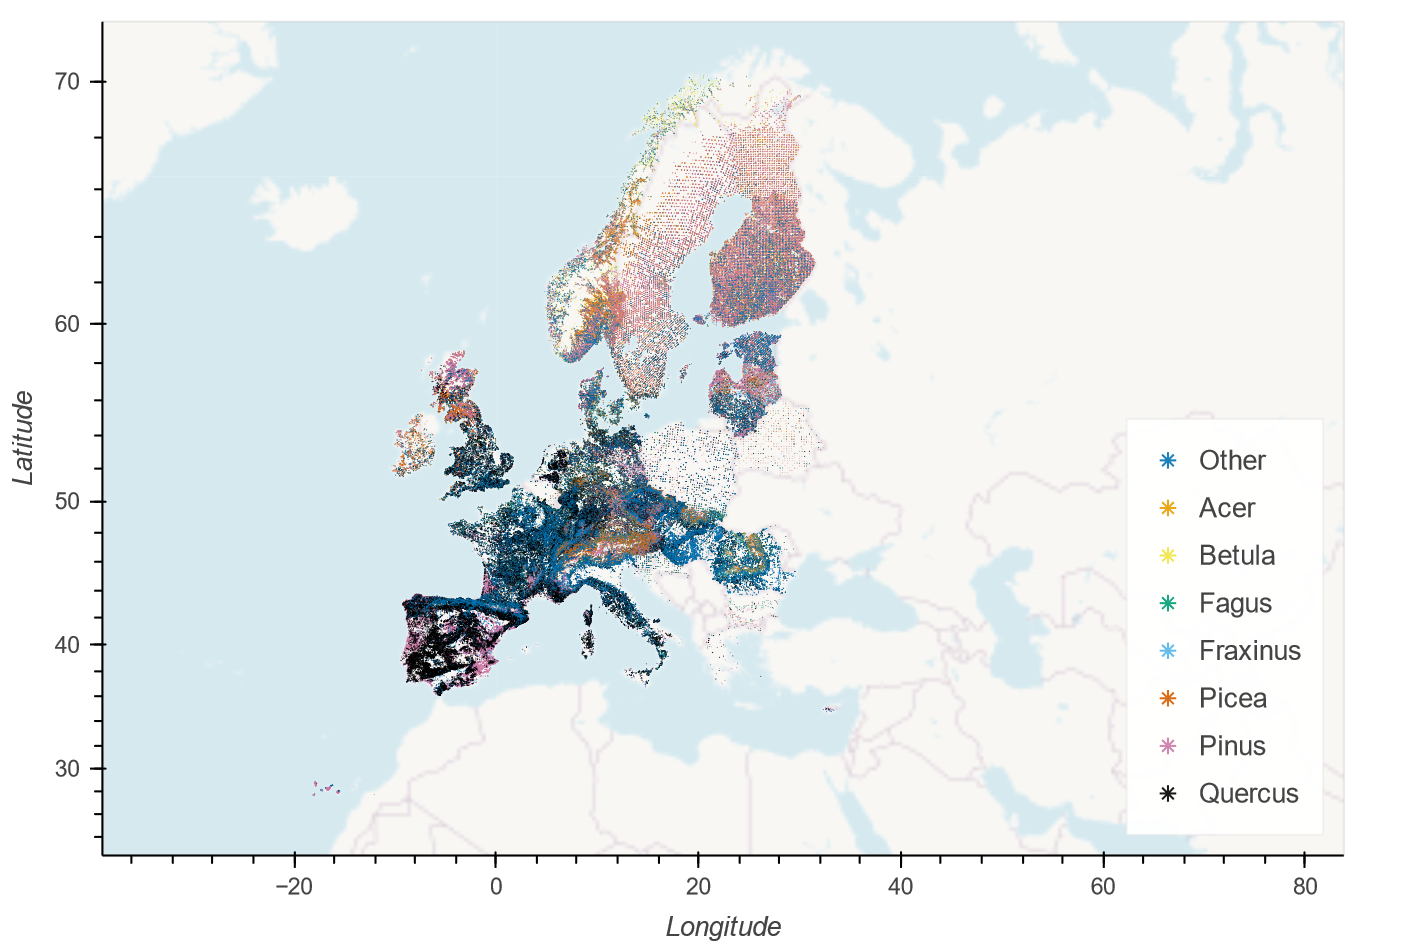
\includegraphics[width=0.9\linewidth]{figures/figures_labels/genus_cutoff_map.png}
    \caption{Map of the most common tree genera in EU-Forest.}
    \label{fig:genus_cutoff_map}
\end{figure}

EU-Forest is a dataset containing tree species and genera for nearly
$250,000$ locations across Europe \cite{eu_forest_data}. Each plot is 1\,km\,×\,1\,km
and may contain multiple tree species and genera.
Fig.\,\ref{fig:genus_cutoff_map} shows the distribution of tree genera in the EU-Forest dataset
across 21 European countries. In this figure, the label 'Other' is an umbrella class for 70 
tree genera with less than 20,000 occurrences each.

Using the EU-Forest dataset to train a convolutional classifier of tree genera with 
Sentinel-2 data offers several significant advantages. 
Firstly, the dataset's high spatial resolution enables fine-grained 
analysis of tree species distribution, which enhances the accuracy of the classifier. 
Its comprehensive coverage across Europe, including diverse forest types and geographical areas, 
allows the model to learn from a wide variety of environments and tree genera.
The rich occurrence data provides detailed information on tree species, 
aiding in precise identification and classification.

\begin{figure}[!thb]
    \centering

    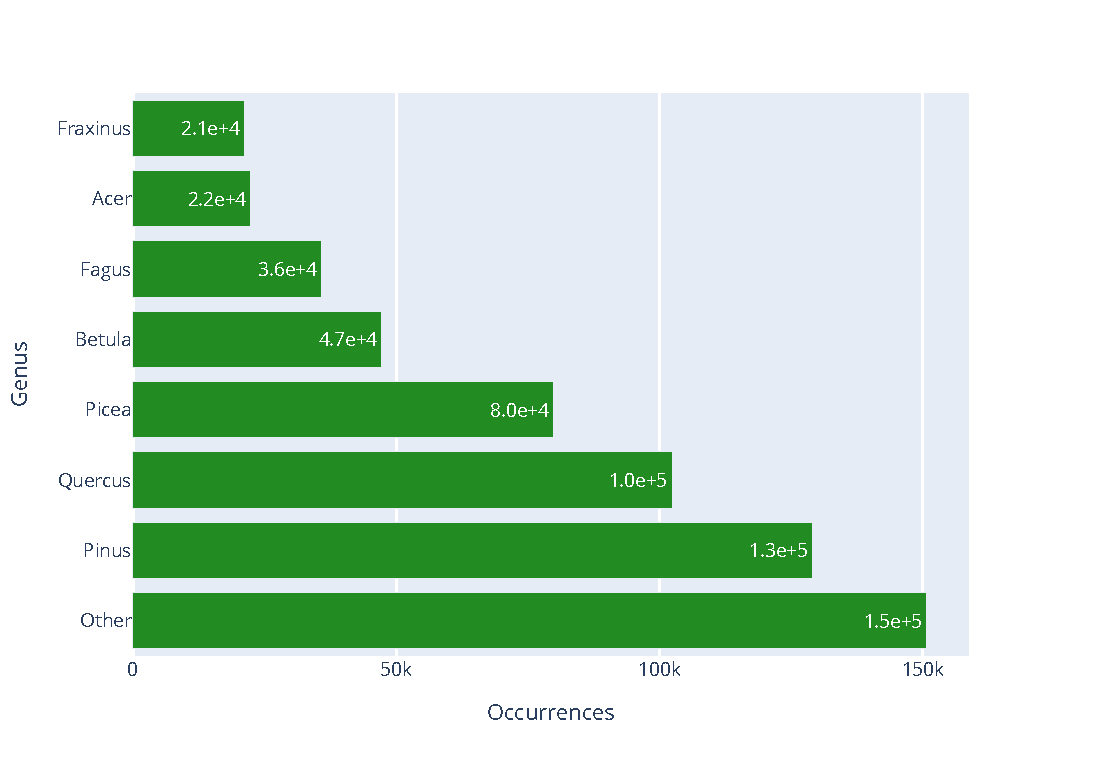
\includegraphics[width=0.48\linewidth, trim={0 0 2cm 0}]{figures/figures_labels/genus_cutoff.pdf}
    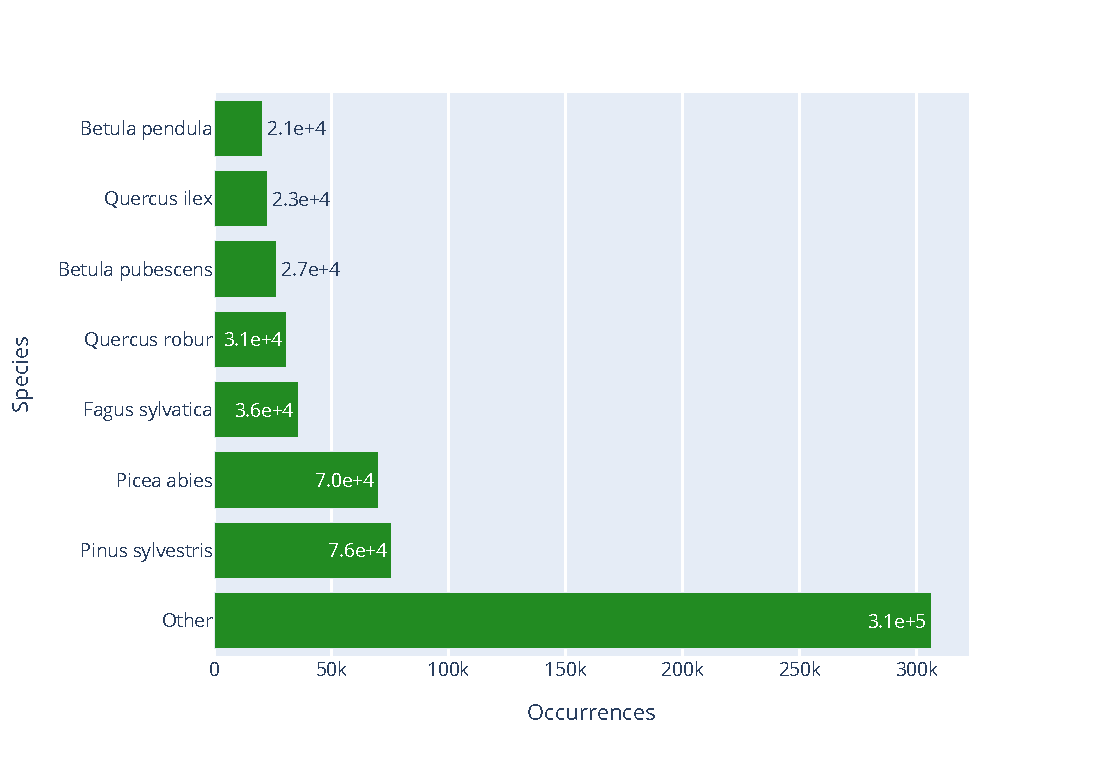
\includegraphics[width=0.48\linewidth, trim={0 0 2cm 0}]{figures/figures_labels/species_cutoff.pdf}

    \caption{Distribution of genera (left) and species (right) in EU-Forest.}
    \label{fig:cutoff_barplots}
\end{figure}

Integration with Sentinel-2 satellite data, which provides high-resolution multispectral images, 
allows for a robust model that leverages both ground-truth data and spectral information.
The dataset, being relatively recent, offers a contemporary snapshot of forest conditions, 
ensuring that the trained model is relevant to current ecological and environmental conditions. 

The plots in Fig.\,\ref{fig:cutoff_barplots} underscore the prevalence of certain genera and species 
in European forests, providing valuable insights for training a convolutional classifier.
The dominance of specific genera and species in the dataset can enhance the classifier's 
ability to accurately identify and classify tree types when combined with Sentinel-2 data.

\begin{figure}[!thb]
    \centering

    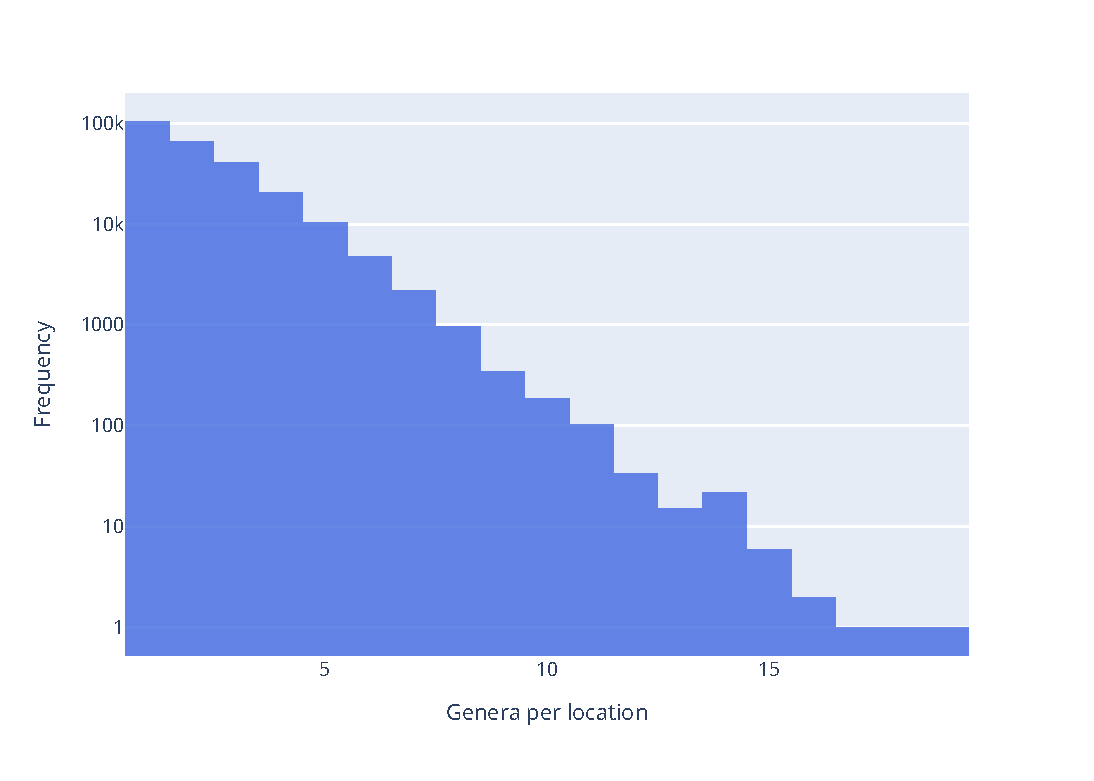
\includegraphics[width=0.48\linewidth, trim={0 0 2cm 0}]{figures/figures_labels/grouped_genus.pdf}%
    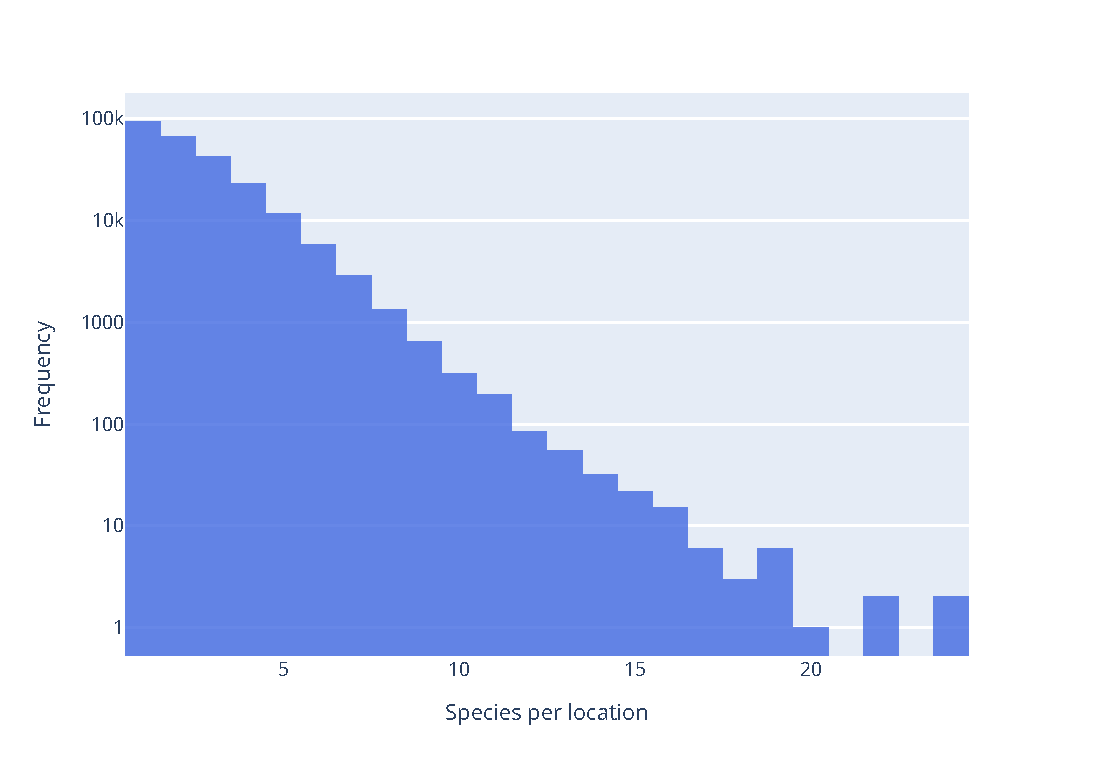
\includegraphics[width=0.48\linewidth, trim={0 0 2cm 0}]{figures/figures_labels/grouped_species.pdf}

    \caption{Distribution of genera (left) and species (right) per location.}
    \label{fig:grouped_histograms}
\end{figure}
 
The plots in Fig.\,\ref{fig:grouped_histograms} reveal a common pattern in biodiversity studies:
most locations are characterized by a limited number of dominant genera and species,
with a smaller number of locations exhibiting higher diversity.
This pattern is important for training a convolutional classifier, as it indicates that
the classifier will often encounter locations with limited genera and species.
However, it must also be capable of handling the less common, more diverse locations.
The high-frequency, low-diversity areas will likely dominate the training process, 
influencing the classifier's ability to generalise across different forest types.

\section{Sentinel-2 Features}

\begin{figure}[ht]
    \centering
    \href{https://sentinels.copernicus.eu/documents/247904/4180891/Sentinel-2-infographic.pdf}
    {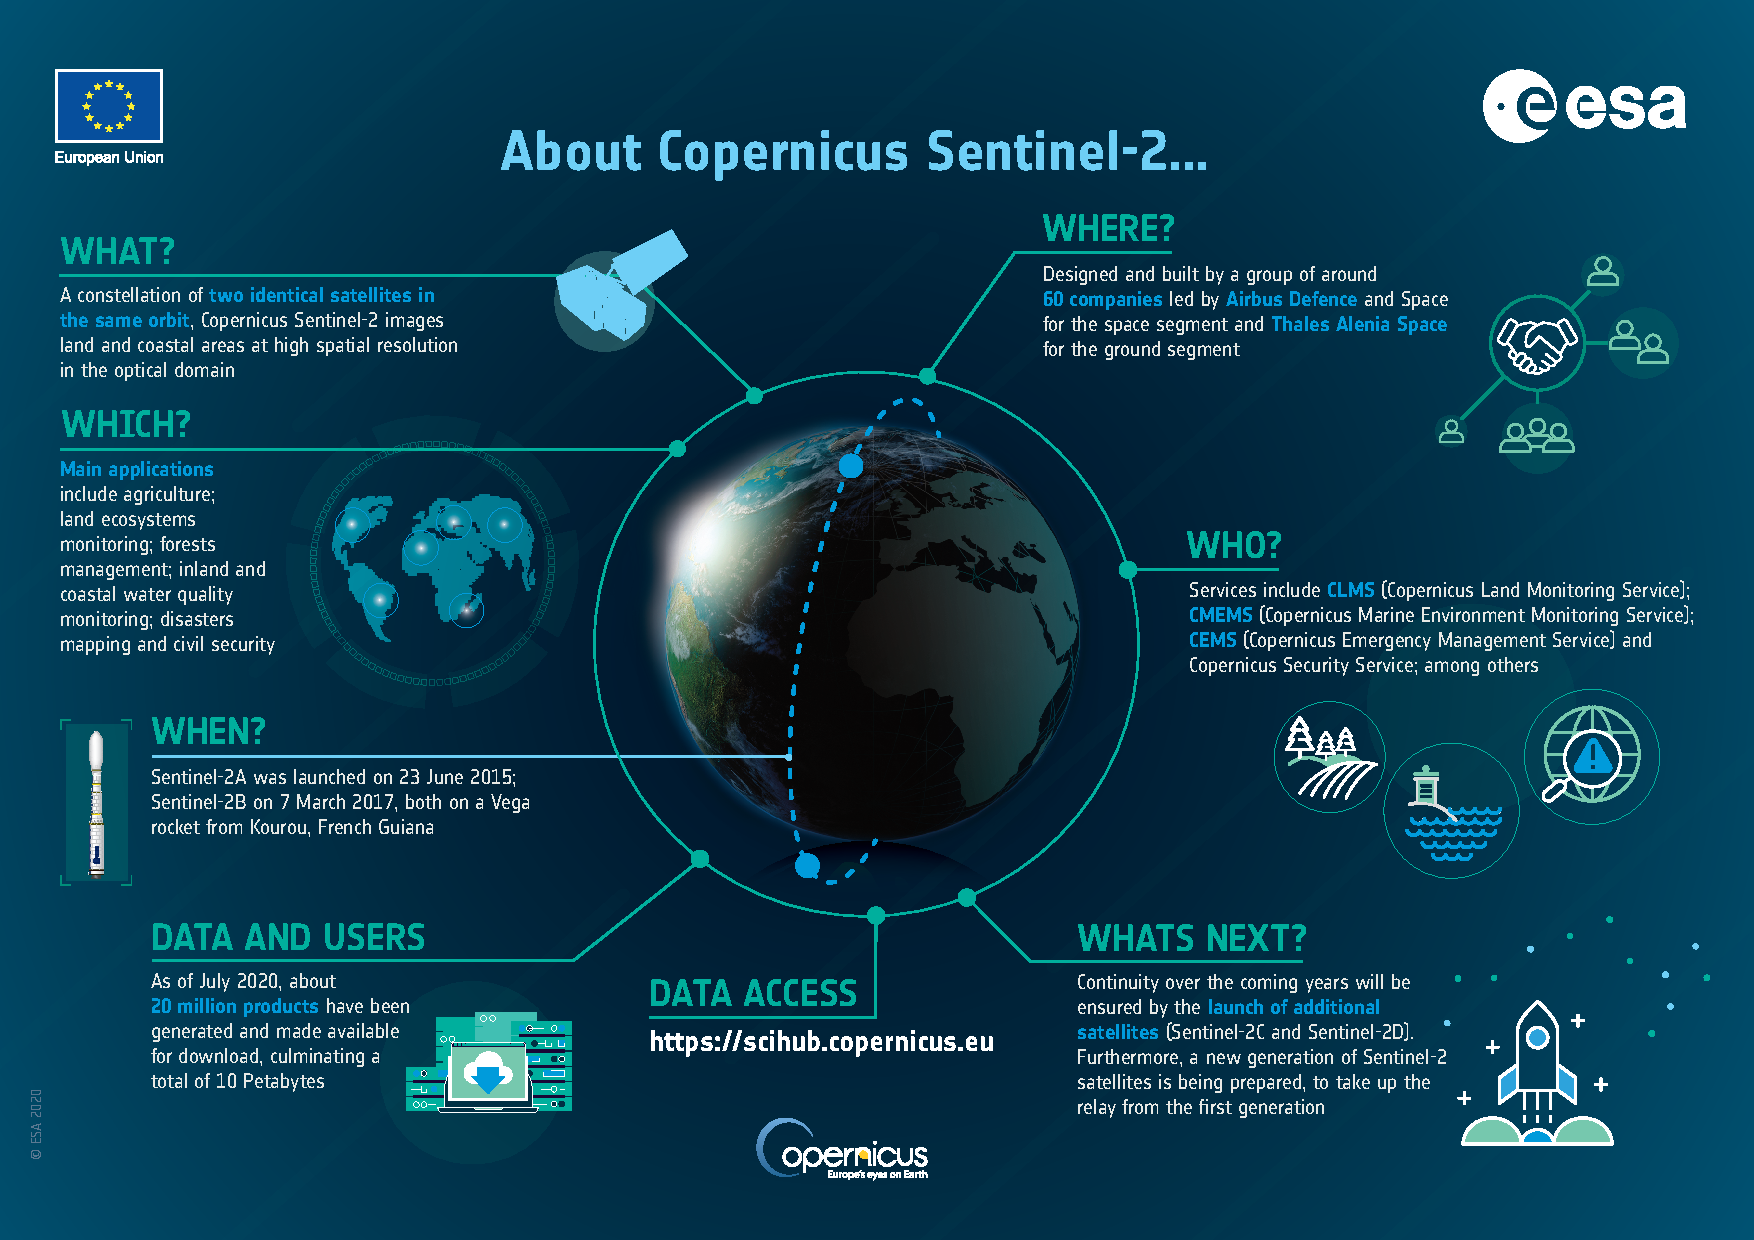
\includegraphics[width=0.9\linewidth]{figures/figures_sentinel/Sentinel-2-infographic.pdf}}
    \caption{
        Sentinel-2 mission infographic. It highlights important facts and 
        achievements of the mission. 
        Courtesy of \href{https://sentinels.copernicus.eu/web/sentinel/missions/sentinel-2}{ESA}.
    }
    \label{fig:sentinel2_info}
\end{figure}

Using Sentinel-2, Fig.\,\ref{fig:sentinel2_info}, specifically the 10-meter and 20-meter resolution bands, 
for training a convolutional classifier of tree genera offers several significant advantages. 
Sentinel-2 provides high-resolution imagery with these bands capturing detailed spatial 
information essential for precise classification tasks.

The 10-meter resolution bands include the visible (red, green, blue) and 
near-infrared (NIR) wavelengths, which are crucial for identifying vegetation 
health and differentiating tree genera based on their reflectance properties. 
The 20-meter resolution bands cover the red-edge, shortwave infrared (SWIR), 
and additional near-infrared regions, further enhancing the classifier's ability
to distinguish between different tree genera by capturing subtle differences in spectral signatures.

The multispectral imaging capability of Sentinel-2, with these selected bands, 
allows for detailed analysis and precise classification of tree genera. 
Each genus reflects and absorbs light differently across these wavelengths, 
providing rich data for the classifier to learn from and accurately identify tree types.

Moreover, Sentinel-2 has a frequent revisit time, with satellites passing over the same 
area every 5 days at the equator. This frequent update cycle is crucial for handling 
cloud cover, as it increases the likelihood of acquiring cloud-free images, 
ensuring that the classifier is trained on clear and usable data.

Sentinel-2 also offers extensive geographical coverage, capturing large areas in each image. 
This comprehensive coverage is essential for training classifiers intended 
for wide-ranging applications across different forest types and regions, 
and it supports the development of global models for tree genus classification.

Additionally, Sentinel-2 data is freely available through the European Space Agency's 
Copernicus program and Google Earth Engine. This open access removes budget constraints, 
making high-quality satellite data accessible for various research and operational purposes.

\begin{figure}[!thb]
    \centering

    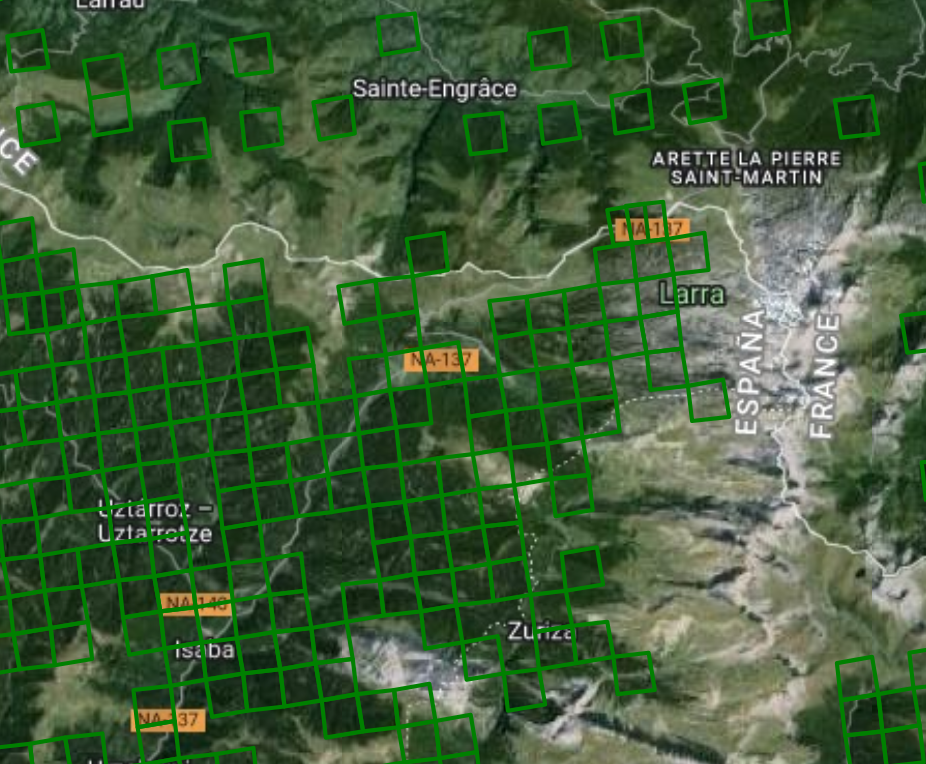
\includegraphics[width=0.48\linewidth]{figures/figures_sentinel/sample_area_earth.png}
    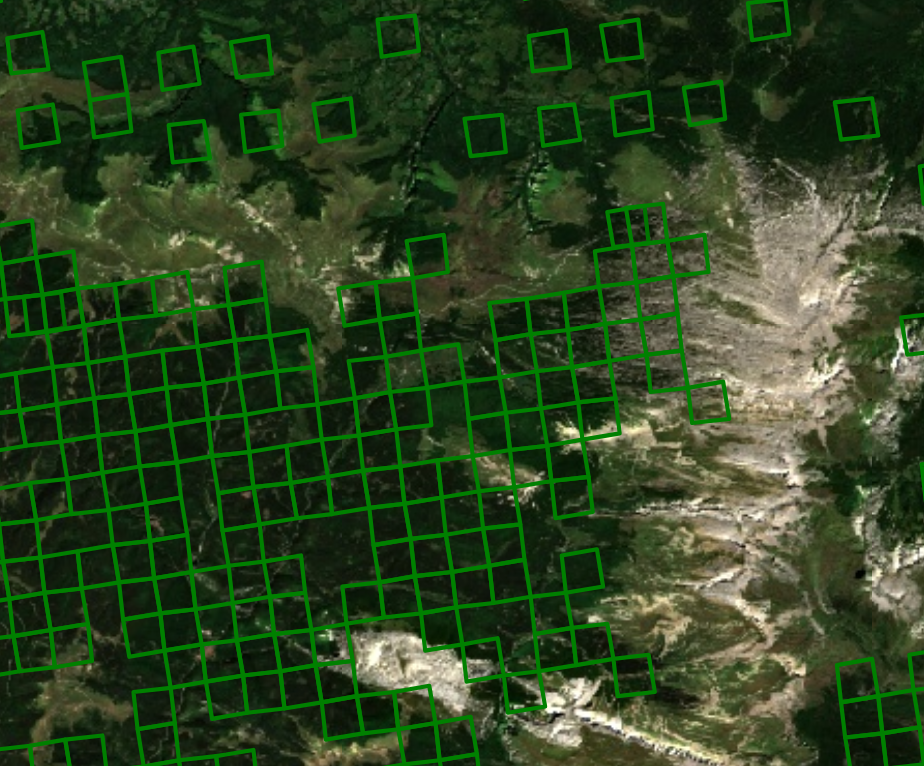
\includegraphics[width=0.48\linewidth]{figures/figures_sentinel/sample_area_sentinel.png}

    \caption{Multiple sample locations overlaid on Google Earth (left) and Sentinel-2 (right) images.}
    \label{fig:_label_sample_area}
\end{figure}

Figs.\,\ref{fig:_label_sample_area} and \ref{fig:label_sample} illustrate the integration of 
high-resolution geographical context with Sentinel-2 satellite data for detailed environmental analysis. 
The grid overlay in the images represents areas for data collection and analysis. 
The left images provide a more detailed geographical context, while the right images show
how Sentinel-2 bands B2, B3, and B4 (blue, green, and red respectively) are structured
 and utilised for spectral analysis.

\begin{figure}[!thb]
    \centering

    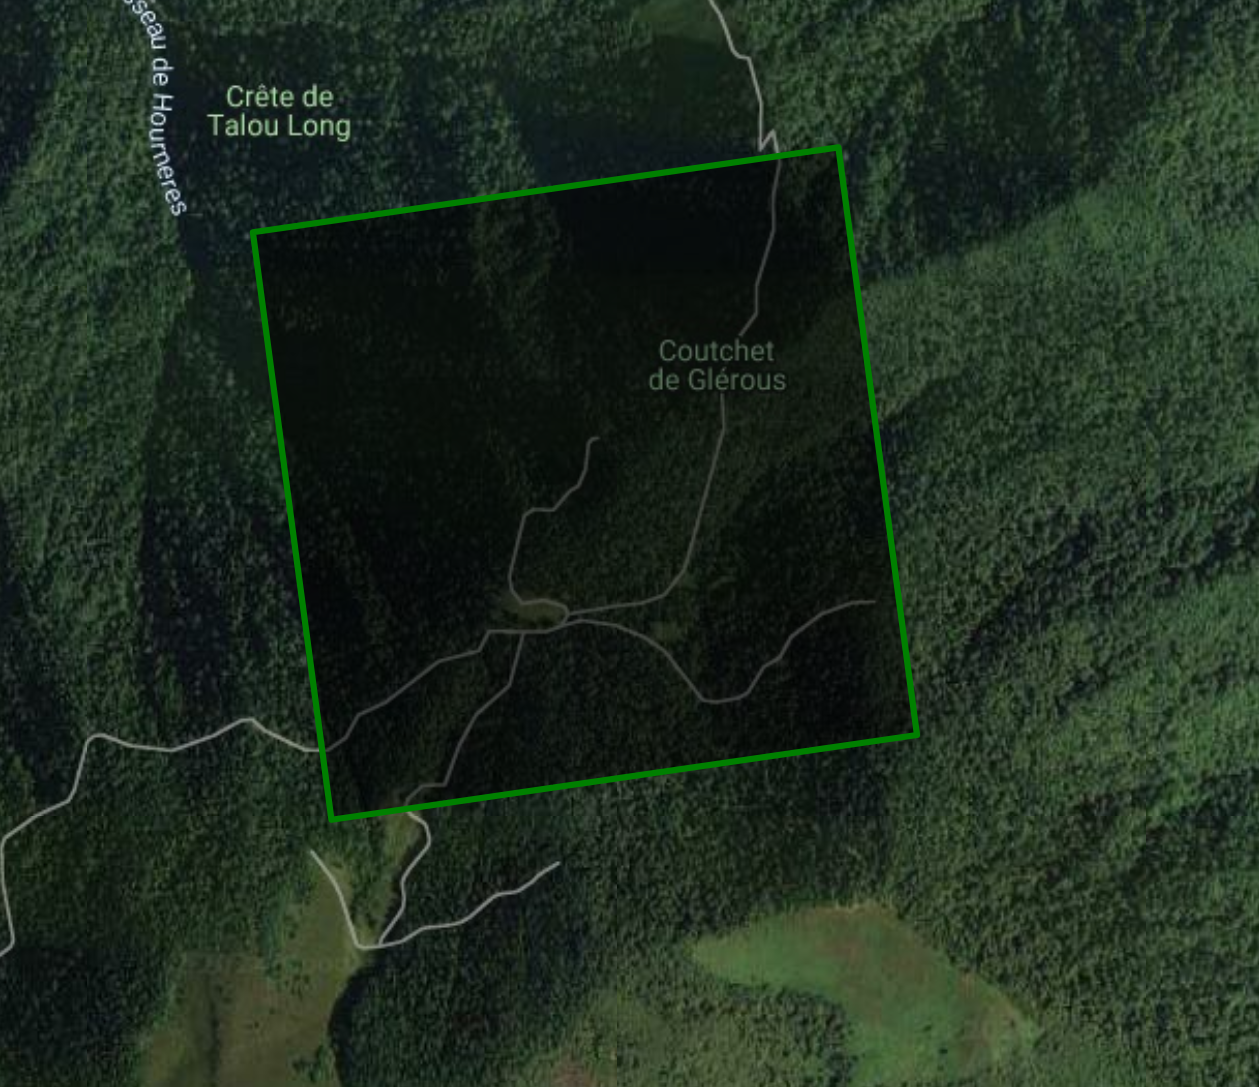
\includegraphics[width=0.48\linewidth]{figures/figures_sentinel/sample_earth.png}
    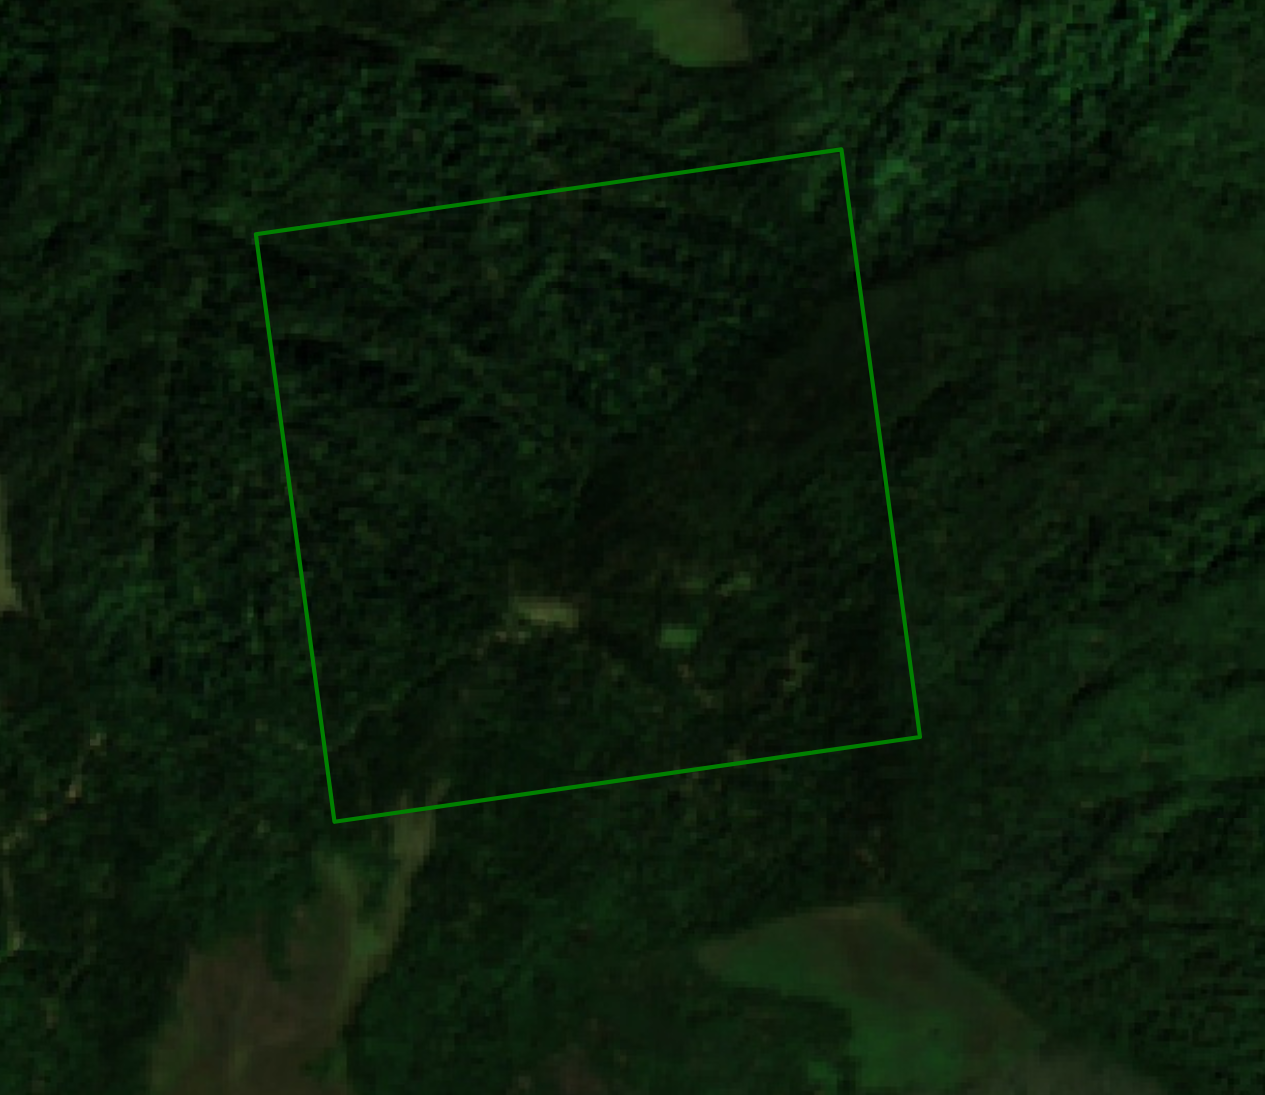
\includegraphics[width=0.48\linewidth]{figures/figures_sentinel/sample_sentinel.png}

    \caption{Sample location overlaid on Google Earth (left) and Sentinel-2 (right) images.}
    \label{fig:label_sample}
\end{figure}